% HA-Expert: A Domain-Adapted Language Model and Evidence-Checked
% Benchmark for Hyaluronan Research
% arXiv preprint manuscript (cs.CL primary; cross-list cs.LG, q-bio.BM).
% Sources: notes/arxiv-draft-v1.md; eval/results/s6-full-report.md;
% eval/verify_summary_v3.md; notes/PROJECT_PLAN.md; model card
% (hf-staging/model-card-sft.md). All reported numbers are taken from
% those records.
% Pre-submission notes: (1) an arXiv endorsement code is still required
% before submission; (2) the reference list is the draft's selected list
% and may be completed at submission time.
\documentclass[11pt]{article}

\usepackage[letterpaper,margin=1in]{geometry}
\usepackage{booktabs}
\usepackage{array}
\usepackage{graphicx}
\usepackage{amsmath}
\usepackage{url}
\usepackage{hyperref}
\hypersetup{colorlinks=true, linkcolor=blue, citecolor=blue, urlcolor=blue}

\title{HA-Expert: A Domain-Adapted Language Model and Evidence-Checked
Benchmark for Hyaluronan Research}

\author{Kunli Liu\\
Independent Researcher, San Francisco Bay Area, USA\\
\href{mailto:liukunli@msu.edu}{liukunli@msu.edu}}

\date{}

\begin{document}
\maketitle


\begin{abstract}
General-purpose LLMs handle specialized fields' literatures
unreliably: fluent answers, often wrong on quantitative details and
confident even when a premise is false. We study one such field ---
hyaluronan (hyaluronic acid, HA) --- and ask how far a single researcher
can go toward a \emph{trustworthy}
domain model. We release (i) a corpus
of 12,306 HA papers ($\sim$126M tokens); (ii) HA-Expert, a
Qwen3-8B-Base model adapted in two stages --- domain-adaptive continued
pretraining (DAPT) on 60M tokens of the corpus, then full-parameter
supervised fine-tuning (SFT) on 12,003 question--answer pairs it
generated itself --- optionally grounded at inference by retrieval over
a 636,959-passage FAISS index; and (iii) HA-Expert-Bench: 240 questions
whose reference answers evidence-restricted LLM verifiers confirmed or
corrected (212 of 240), including 15 adversarial ``trap'' questions. In a four-cell ablation, SFT doubles the base model
(0.300 $\rightarrow$ 0.601); retrieval is the largest single lever
(base+RAG 0.710; traps 0.267 $\rightarrow$ 0.867); and SFT and RAG do
\textbf{not} compose additively (0.662): a model never trained on
retrieved context collapses into citation-marker loops (5 of 240
responses) and inherits its teacher's repetition habit.
\end{abstract}

\section{Introduction}
\label{sec:intro}

Hyaluronan is a linear glycosaminoglycan of repeating
$\beta$-1,4-glucuronic-acid / $\beta$-1,3-$N$-acetylglucosamine
disaccharides. Practitioners' knowledge ---
molecular-weight-dependent biology, receptor interactions, chemical
modification, production, clinical dosing --- is spread across thousands
of chemistry, materials, and medical papers.

General-purpose LLMs promise an interface to such a literature, but our
probes found three systematic failures: \emph{behavior} (base model
continued prompts with invented follow-up questions), \emph{epistemic
stance} (assent to false premises --- HA is a protein polymer; HA
solutions are Newtonian fluids), and \emph{verifiability} (quantitative
claims with no checkable source).

We address them with the standard toolkit (continued pretraining,
instruction tuning, retrieval) under three small-lab constraints: (1) one
rented GPU; (2) no paid teacher: supervision
self-generated, then filtered; (3) trusted evaluation: reference answers
\emph{checked against source text}, not merely model-written. Constraint
(2) makes this a self-distillation exercise, whose risks we measure, not
assume away.

Contributions: the corpus, the model (Section~\ref{sec:methods}), and
the benchmark. The headline result is
negative: in the four-cell ablation, fine-tuning doubles the base score,
retrieval on the untrained base is worth still more, yet the combination
underperforms retrieval alone (Section~\ref{sec:analysis}).

\section{Related Work}
\label{sec:related}

We assemble standard components, not new algorithms; the interest is
their interaction. Continued pretraining plus full-parameter SFT is the
established route to domain language models, instantiated here with
Qwen3-8B-Base and Qwen3-Embedding-0.6B~\cite{qwen3} in Transformers and
TRL~\cite{transformers,trl}, with NEFTune noise~\cite{neftune} and
general-domain replay~\cite{fineweb}. Self-generated instruction data
risks distilling the generator's errors and habits unchecked, mitigated
by a grounding filter (Section~\ref{sec:sft-data}) and an evaluation
designed to expose what survives it. Dense retrieval
(FAISS~\cite{faiss}) is the standard remedy for such failures. Domain
benchmarks commonly ship un-re-checked model-written keys whose errors
judges inherit; ours are evidence-verified (Section~\ref{sec:bench}).

\section{Corpus}
\label{sec:corpus}

\textbf{Harvest and cleaning.} Harvesting PubMed Central's open-access
subset gave 16,642 records, 12,945 with retrievable JATS XML full text. Plain-text conversion, deduplication
(exact and near), and language/length filtering left \textbf{12,306
papers, $\approx$126M tokens}.

\textbf{Holdout.} Thirty review papers were set aside \emph{before} any
processing and excluded from all downstream stages (DAPT, SFT data,
index), so questions derived from them measure generalization, not
recall.

\textbf{DAPT sets.} A \emph{core set} of 4,952 papers (60.0M tokens) and
an \emph{anneal set} of 498 papers (5.7M tokens) of reviews and methods
papers, placed last, with 12\% FineWeb-Edu replay.

\textbf{What the model reads.} Two samples from the released artifacts
show the actual inputs. A corpus record (PMC10000474, \emph{Foods},
2023) begins:
\begin{quote}\small
Hyaluronic acid (HA) is now widely known for its ability to bind water
and impart texture. The combined effects of HA and kappa-carrageenan
(KC) have not yet been investigated, though. In this study, we looked at
the synergistic effects of HA and KC (concentrations of 0.1 and 0.25\%,
and ratios of 85:15, 70:30, and 50:50 for each concentration) on the
rheological properties, heat stability, protein phase separation,
water-holding capacity, emulsification \ldots
\end{quote}
Retrieval chunks are $\approx$900-character windows cut across sentence
boundaries; a chunk from the same paper begins mid-word:
\begin{quote}\small
ser protein phase separation and a higher water-holding capacity than
when HA and KC were utilized separately. Similarly, for the sample with
a 0.1\% concentration, the combination of HA + KC blends demonstrated a
synergistic impact with greater emulsifying activity and stability. The
samples with a concentration of 0.25\% did not exhibit this synergistic
effect \ldots
\end{quote}
DAPT consumes record text like the first sample; SFT pairs are generated
from such passages (Section~\ref{sec:sft-data}); at inference, chunks
like the second are prepended to the question
(Section~\ref{sec:rag}). Full readable samples are in
\texttt{examples/sample-data.md} in the repository.

\section{Methods}
\label{sec:methods}

Three stages (DAPT, SFT on self-generated data, retrieval-augmented
inference), then evaluation on HA-Expert-Bench
(Section~\ref{sec:bench}; Figure~\ref{fig:pipeline}) --- all on one
rented GPU.

\begin{figure}[t]
\centering
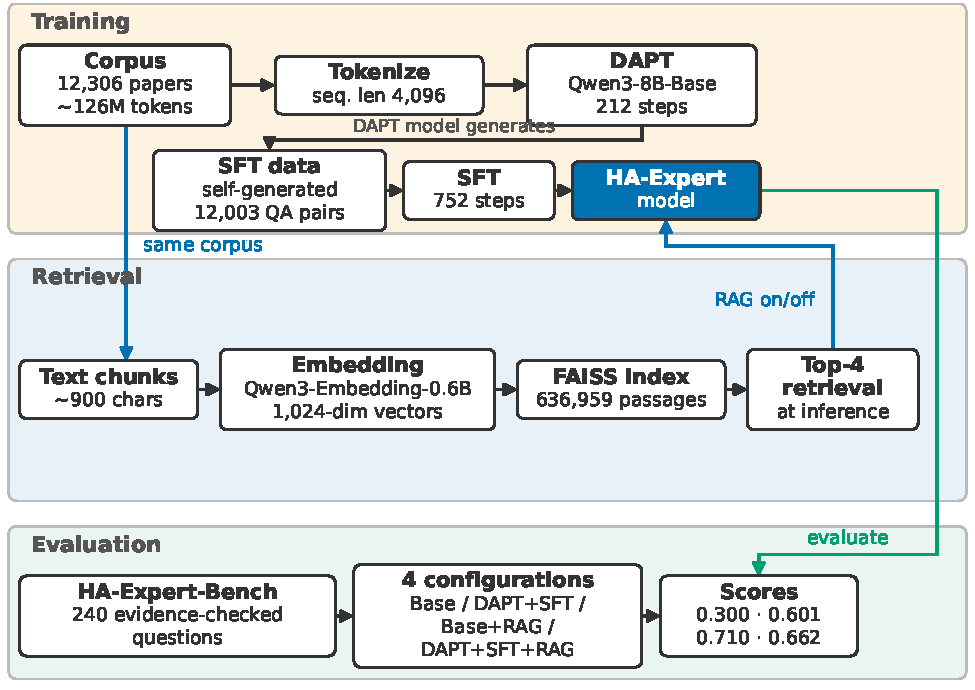
\includegraphics[width=\textwidth]{figs/fig1-pipeline.pdf}
\caption{The HA-Expert pipeline. \textbf{Training:} the 12,306-paper
corpus is tokenized for DAPT of Qwen3-8B-Base, which then generates its
own grounding-filtered SFT data. \textbf{Retrieval:} the corpus is
chunked into a FAISS index of 636,959 passages; the top-4 are prepended
at inference (RAG on; off: parameters alone). \textbf{Evaluation:} all
four configurations are scored on HA-Expert-Bench's 240 evidence-checked
questions.}
\label{fig:pipeline}
\end{figure}

\subsection{Domain-adaptive pretraining (DAPT)}
\label{sec:dapt}

Full-parameter continued pretraining of Qwen3-8B-Base~\cite{qwen3} on the
Section~\ref{sec:corpus} DAPT sets: documents chunked into
4,096-token sequences (legacy block packing), SDPA attention;
effective batch 128 sequences (8 $\times$ gradient accumulation 16) =
524,288 tokens/step; learning rate $1\times10^{-5}$, cosine decay; 212
steps ($\approx$111M tokens) in 5\,h 34\,min on a single RTX PRO 6000
(96\,GB); final loss $\approx$1.55. On a 63-question development split,
DAPT tied base on auto-graded items (5/6) yet repaired knowledge traps it
missed: it changed what the model \emph{knows}, not how it
\emph{behaves} --- motivating SFT.

\subsection{Self-generated SFT data}
\label{sec:sft-data}

The DAPT model served as its own teacher:
\begin{enumerate}
\item Serve the DAPT model locally with vLLM~\cite{vllm}.
\item Sample passages, excluding the 30 holdout papers
(Section~\ref{sec:corpus}).
\item Generate a question--answer pair per passage, anchored to the
passage.
\item Retain only pairs whose answer is \emph{grounded} in the passage
(content-word overlap $\geq 0.55$); deduplicate.
\end{enumerate}
Two rounds: 5,403 + 6,600 retained pairs --- \textbf{12,003
examples} --- filtered for topical attestation, not truth
(Section~\ref{sec:limitations}).

\subsection{Supervised fine-tuning}
\label{sec:sft-train}

Full-parameter SFT in prompt/completion format, loss on the completion
only: learning rate $1\times10^{-5}$, 2 epochs (752 steps), NEFTune
noise~\cite{neftune} 5.0, 8-bit Adam; final train loss 1.214 in
$\approx$19 minutes. The base model's signature pathology (inventing
follow-up questions) disappeared.

\subsection{Retrieval-augmented inference (RAG)}
\label{sec:rag}

All 12,306 papers were chunked by merging paragraphs to $\approx$900
characters (150-character overlap on long paragraphs) and embedded with
Qwen3-Embedding-0.6B (1,024-dimensional) into a FAISS
IndexFlatIP~\cite{faiss} index of \textbf{636,959 passages} (holdout
absent). At inference the top-4 passages are prepended with citation
markers [1]--[4] the model is instructed to cite. Decoding: demo,
repetition penalty 1.05 (largely suppresses the repetition failure mode,
Section~\ref{sec:analysis}); benchmark, plain greedy, so aids cannot
mask measured behavior.

\section{HA-Expert-Bench}
\label{sec:bench}

\subsection{Composition}

HA-Expert-Bench: 240 questions in seven categories
(basics; history/industry; synthesis/chemistry; modification/derivatives;
molecular-weight biology/receptors; nano-delivery;
experimental/clinical topics) and four formats
(Table~\ref{tab:benchcomp}). \emph{Trap} questions embed a false premise
an expert should reject (premise rejection, Section~\ref{sec:intro}).

\begin{table}[t]
\centering
\begin{tabular}{lcll}
\toprule
Format & $n$ & Grading & Notes \\
\midrule
Open & 195 & LLM judge & free-form answers \\
Quantitative & 20 & automatic & numeric tolerance \\
Trap & 15 & LLM judge & false premise to reject \\
Multiple-choice & 10 & automatic & exact option letter \\
\midrule
Total & 240 & & \\
\bottomrule
\end{tabular}
\caption{HA-Expert-Bench composition. Judge-graded items use the
correct / partial / wrong rubric of Section~\ref{sec:grading}, scored
1.0 / 0.5 / 0.0 against the evidence-checked reference key.}
\label{tab:benchcomp}
\end{table}

\subsection{Evidence-checked answer keys}
\label{sec:keys}

Each draft key passed an evidence-restricted protocol: verifiers with
only an evidence pack could \emph{confirm} a key, \emph{correct} it
(quoting the decisive passage), or mark it \emph{uncertain}. Round one
(packs
traced to source papers for 38 questions, keyword-retrieved for 202): 118
verified, 19 corrected, 103 uncertain. Round two (the 103, against top-6
vector-retrieved passages, Section~\ref{sec:rag}): 72 verified, 3
corrected, 28 still uncertain. Released v3 set: 190 verified, 22
corrected --- \textbf{212 of 240 (88.3\%) evidence-settled} --- 28
(11.7\%) flagged uncertain. Only three keys changed in round two (B22,
F07; G14), and re-scoring under v3 changed no auto-grade and no G14
verdict.

\subsection{Grading protocol}
\label{sec:grading}

Multiple-choice: exact option letter; quantitative: numeric tolerance.
Open and trap items are graded by an LLM judge shown question,
evidence-checked reference answer, and response, returning correct /
partial/wrong (1.0/0.5/0.0). The judge was the SFT model itself,
served locally (\$0; bias: Section~\ref{sec:limitations}). Mitigation:
fixed-key anchoring, plus the 30 automatic items as a judge-free control
(Section~\ref{sec:experiments}). Unparseable outputs were re-judged in a
retry pass (scores moved by at most 0.004).

\section{Experiments and Results}
\label{sec:experiments}

\subsection{Protocol}

Four cells: base (Qwen3-8B-Base), adapted (DAPT+SFT), each also with
retrieval. All responses used greedy decoding
(temperature 0, maximum 512 tokens) on a single RTX PRO 6000 (96\,GB).
Unparseable-after-retry items remained ungraded --- 13
(base), 23 (DAPT+SFT), 2 (base+RAG), 21 (DAPT+SFT+RAG) --- leaving
$n = 227$, $217$, $238$, $219$. Gaps below $\approx$0.02 are noise.

\begin{table}[t]
\centering
\begin{tabular}{lccccc}
\toprule
Cell & Overall & MCQ (10) & Quant.\ (20) & Open (195) & Trap (15) \\
\midrule
Qwen3-8B-Base        & 0.300 & 0.800 & 0.250 & 0.282 & 0.267 \\
+ DAPT \& SFT        & 0.601 & \textbf{0.900} & 0.300 & 0.631 & 0.500 \\
+ RAG                & \textbf{0.710} & \textbf{0.900} & 0.450 & \textbf{0.719} & \textbf{0.867} \\
+ DAPT \& SFT \& RAG & 0.662 & 0.700 & \textbf{0.550} & 0.676 & 0.633 \\
\bottomrule
\end{tabular}
\caption{HA-Expert-Bench results (240 questions; means over graded items,
$n$ per cell as in Section~\ref{sec:experiments}). Bold marks the best
score in each column. Three facts organize the table: fine-tuning doubles
the base model; retrieval on the \emph{base} model beats the full
training pipeline without it; and the combination underperforms
retrieval alone on open and trap questions while posting the best
quantitative score. On the 30 auto-graded items alone (no judge):
0.433 / 0.500 / 0.600 / 0.600, same cell order.}
\label{tab:main}
\end{table}

\begin{figure}[t]
\centering
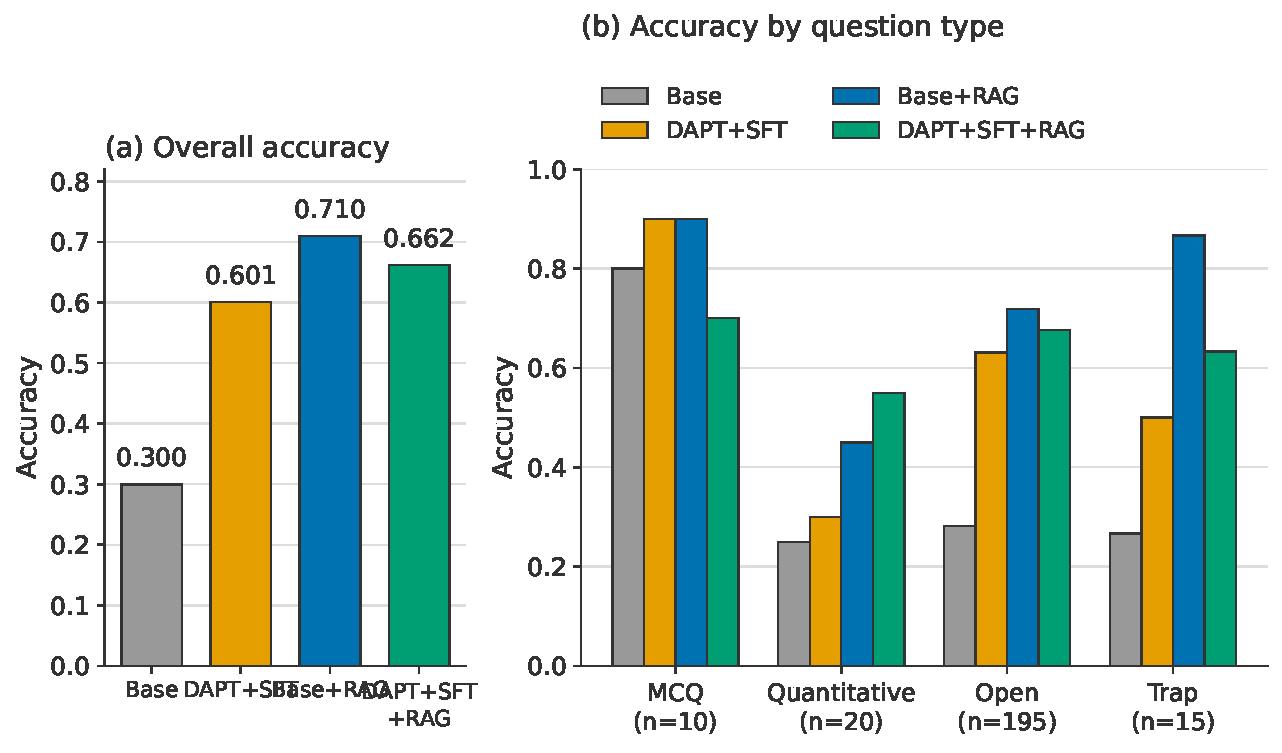
\includegraphics[width=\textwidth]{figs/fig2-results.pdf}
\caption{HA-Expert-Bench results by configuration (240 questions;
graded $n$ per Section~\ref{sec:experiments}). (a) Overall: fine-tuning
doubles the base model (0.300 $\rightarrow$ 0.601); retrieval alone is
worth more (0.710); the two do not compose additively (0.662). (b) By
type: retrieval's largest effect is on traps (0.267 $\rightarrow$
0.867); best quantitative: combined cell (0.550). Colors match
Figure~\ref{fig:failures}.}
\label{fig:results}
\end{figure}

\subsection{Fine-tuning doubles the base model}

DAPT+SFT scores 0.601 against base 0.300 (Table~\ref{tab:main},
Figure~\ref{fig:results}), the gain largest where the base deficit was
behavioral (open questions: 0.282 $\rightarrow$ 0.631; the model now
answers instead of continuing the prompt; cf.\ Section~\ref{sec:dapt}).
Trap accuracy improves
(0.267 $\rightarrow$ 0.500) but remains unreliable.

\subsection{Retrieval is the largest single lever}

Base+RAG scores 0.710 --- above the full pipeline without retrieval
(0.601). The effect is largest where parametric knowledge is least
reliable: trap accuracy rises 0.267 $\rightarrow$ 0.867, and both
parametric trap failures (G01, G13) are corrected by both retrieval
cells. A false premise is hard to reject from memory, easy with the
contradicting passage in the prompt.

\subsection{SFT and RAG interfere}

DAPT+SFT+RAG (0.662) trails base+RAG despite dominating it without
retrieval. The deficit concentrates in the judged formats --- open (0.676
vs.\ 0.719), trap (0.633 vs.\ 0.867) --- but not uniformly: the combined
cell is best on quantitative questions (0.550 vs.\ 0.450). On the 30
auto-graded items it \emph{ties} base+RAG (0.600 each): the headline gap
lives in the judged formats, not the objective subset.

\section{Analysis}
\label{sec:analysis}

\subsection{Mechanism 1: a train/test format mismatch}

The SFT data (Section~\ref{sec:sft-data}) contains only bare
question$\rightarrow$answer pairs, so the fine-tuned model never saw the
RAG format (question + four retrieved passages + citation instruction).
On 5 of 240 such inputs it collapses into a
\emph{citation-marker loop} (``[1] [4] [2] [3] [1] [4] [2] [3]
$\ldots$''), scoring zero on questions it answers correctly without
retrieval. The failure is diagnostic: the markers are
the most salient novel tokens in the unseen format, and a model trained
to continue its prompt's pattern continues them --- a
\emph{training-data omission}, not retrieval hurting a well-matched
model (fix: Section~\ref{sec:future}).

\subsection{Mechanism 2: repetition inherited through self-distillation}

\emph{Heavy repetition} (defined in Figure~\ref{fig:failures}) appears
in 35 of 240 DAPT+SFT responses vs.\ 10 of 240 for base, retrieval
lowering both (7, 22 of 240). Because the teacher \emph{was} the DAPT
model itself (Section~\ref{sec:sft-data}), its repetition habit was
distilled into the student --- self-distillation transmits even
degenerate behavior, unscreened by a content-word grounding filter.
Repetition is decode-sensitive --- largely suppressed in the demo
(Section~\ref{sec:rag}) --- but the benchmark's unaided greedy decoding
measures it.

\begin{figure}[t]
\centering
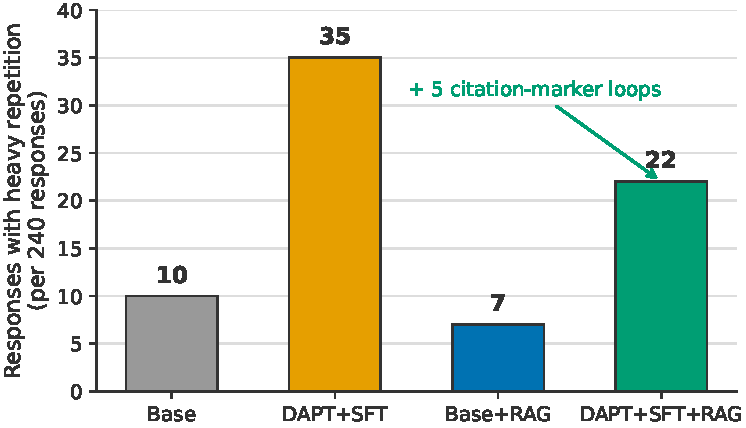
\includegraphics[width=0.85\textwidth]{figs/fig3-failure-modes.pdf}
\caption{Failure-mode counts per configuration (240 responses each,
greedy decoding). \emph{Heavy repetition}: a 30-character block repeated
at least $5\times$ in one response. Self-generated fine-tuning data more
than triples the base count (10 $\rightarrow$ 35): the teacher's habit,
distilled; retrieval lowers both counts. The annotation marks Mechanism
1's 5 citation-marker loops (DAPT+SFT+RAG only).}
\label{fig:failures}
\end{figure}

\subsection{Case studies}

Both mechanisms appear in pure form on trap items. \textbf{G13}
(``HA solutions are Newtonian fluids, so viscosity is a single
constant''): the SFT model assents, repeating itself (``Yes, HA
solutions are simple Newtonian fluids\ldots''); with retrieval it
corrects the premise (``No, HA solutions are not simple Newtonian
fluids\ldots''). \textbf{G09} (highest-MW HA always best for joint
injections): the SFT model rejects the absolute; SFT+RAG degenerates
into a citation-marker loop (``[1] [4] [2] [3] $\ldots$''). Retrieval
rescues G13 and destroys G09.

\begin{table}[t]
\centering
\begin{tabular}{lcccc}
\toprule
Trap & Base & SFT & Base+RAG & SFT+RAG \\
\midrule
G01 & wrong   & wrong   & correct & correct \\
G02 & wrong   & wrong   & correct & wrong \\
G03 & wrong   & wrong   & correct & partial \\
G04 & partial & correct & correct & correct \\
G05 & partial & correct & correct & correct \\
G06 & partial & correct & correct & wrong \\
G07 & partial & correct & partial & partial \\
G08 & partial & correct & correct & correct \\
G09 & wrong   & correct & partial & wrong \\
G10 & wrong   & ungraded & partial & partial \\
G11 & wrong   & wrong   & correct & correct \\
G12 & correct & ungraded & correct & wrong \\
G13 & wrong   & wrong   & correct & correct \\
G14 & wrong   & wrong   & correct & correct \\
G15 & partial & partial & partial & correct \\
\bottomrule
\end{tabular}
\caption{Per-question verdicts on the 15 trap items. Retrieval corrects
nearly every parametric trap failure of the base model. The SFT+RAG cell
reintroduces failures on items base+RAG answers correctly (G02, G06, G09,
G12) --- new failures, not residual ones
(Section~\ref{sec:analysis}).}
\label{tab:traps}
\end{table}

\section{Limitations}
\label{sec:limitations}

\textbf{The judge is one of the contestants.} Open and trap items are
graded by the SFT model itself (Section~\ref{sec:grading}); fixed-key
anchoring and the judge-free auto-graded control bound, but do not
eliminate, the distortion.
\textbf{Residual key uncertainty.} 28 of 240 keys (11.7\%) remain
uncertain drafts; verification \emph{changed} 22 of 240 keys (9\%) --- an
unchecked key set would have carried that error rate silently into every
score --- including the drafting model's own.
\textbf{Small cells.} Multiple-choice rests on $n=10$: the SFT+RAG dip
(0.700 vs.\ 0.900) is two questions; no conclusion drawn. Trap verdicts
($n=15$) are in Table~\ref{tab:traps}.
\textbf{Attestation, not truth.} The grounding filter's overlap
($\geq 0.55$) shows an answer is about a real passage, not that it states
it correctly, so SFT data can encode teacher errors
(Section~\ref{sec:sft-data}); factual contamination of the same kind
(cf.\ repetition inheritance, Section~\ref{sec:analysis}) cannot be
excluded without expert audit. \textbf{Decoding
and scale.} All results are a single greedy run, and repetition is
decode-sensitive, so Mechanism 2's size is a property of
model-plus-decoding; and one 8B model in one domain makes the pipeline
and failure analysis --- not any absolute score --- the transferable
claim. \textbf{Replicability.} Only the corpus query is HA-specific
(harvest $\rightarrow$ clean $\rightarrow$ DAPT $\rightarrow$ self-SFT
$\rightarrow$ bench $\rightarrow$ ablation): a template for
small fields with open-access literatures, and a warning worth having
\emph{before} combining SFT with retrieval.

\section{Future Work}
\label{sec:future}

One fix per mechanism (Section~\ref{sec:analysis}):
\emph{retrieval-formatted SFT data} for the format mismatch --- examples
in the exact inference format (question + retrieved excerpts + cited
answer), predicted to move the combined cell above base+RAG;
\emph{repetition filtering} of teacher outputs for the inheritance,
screening pairs by the failure's operational definition. Evaluation-side:
re-grade with an external judge and settle the 28 uncertain keys.

Beyond hyaluronan, three directions follow. \emph{Other domains:} the
pipeline is domain-agnostic apart from the corpus query
(Section~\ref{sec:limitations}), so the same recipe applies to other
literature-bound fields --- heparin and other glycosaminoglycans, or
bioconjugation chemistry. \emph{Ideation:} the released model already
proposes novel research ideas and expands them into structured plans
with hypotheses and experimental methods; adding corpus-scale novelty
checking against the literature would turn that capability into a
research tool. \emph{Review:} a model with verified command of a field's
literature could serve as a first-pass reviewer of new submissions,
checking claims against that literature --- a use that, like ideation,
needs evidence-checked evaluation before it can be trusted.

\section{Data and Code Availability}
\label{sec:availability}

\begin{itemize}
\item Code, corpus, benchmark (v3 keys + verification status), results:
\url{https://github.com/liukunli001/hyaluronan-expert-llm}
\item Weights: \url{https://huggingface.co/liukunli/ha-expert-qwen3-8b}
(SFT model) and
\url{https://huggingface.co/liukunli/ha-expert-qwen3-8b-dapt} (DAPT
checkpoint)
\item Retrieval index:
\url{https://huggingface.co/datasets/liukunli/ha-expert-index}
\item Demo: \url{https://huggingface.co/spaces/liukunli/ha-expert-demo}
\item Corpus release: GitHub Release \texttt{v0.1-data}.
\end{itemize}

\section*{Acknowledgements}

Thanks to the open-access publishers whose PMC deposits made the corpus
possible, and to the Qwen, Hugging Face, vLLM, and FAISS communities.

\begin{thebibliography}{9}

\bibitem{qwen3}
Qwen Team.
\newblock \emph{Qwen3 Technical Report}.
\newblock Alibaba Group, 2025.

\bibitem{transformers}
Wolf, T., et al.
\newblock Transformers: State-of-the-Art Natural Language Processing.
\newblock In \emph{Proceedings of EMNLP 2020: System Demonstrations}.

\bibitem{trl}
von Werra, L., et al.
\newblock \emph{TRL: Transformer Reinforcement Learning}.
\newblock Hugging Face library, 2023.

\bibitem{neftune}
Jain, N., et al.
\newblock NEFTune: Noisy Embeddings Improve Instruction Finetuning.
\newblock \emph{arXiv:2310.05914}, 2023.

\bibitem{fineweb}
Penedo, G., et al.
\newblock The FineWeb Datasets: Decanting the Web for the Finest Text Data
at Scale.
\newblock In \emph{Advances in Neural Information Processing Systems
(NeurIPS)}, 2024.
\newblock (FineWeb-Edu subset used for replay.)

\bibitem{vllm}
Kwon, W., et al.
\newblock Efficient Memory Management for Large Language Model Serving
with PagedAttention.
\newblock In \emph{Proceedings of SOSP}, 2023.

\bibitem{faiss}
Johnson, J., Douze, M., and J\'egou, H.
\newblock Billion-Scale Similarity Search with GPUs.
\newblock \emph{IEEE Transactions on Big Data}, 7(3):535--547, 2021.

\end{thebibliography}

\end{document}
